\documentclass[12pt]{article}

% Packages
\usepackage{tikz}
\usepackage[utf8]{inputenc}
\usepackage{graphicx}
\usepackage{enumerate}
\usepackage{tabularx}
\usepackage{longtable}
\usepackage{booktabs}
\usepackage{caption}
\usepackage{placeins}
\usepackage{float}
\usepackage{multirow}
\usepackage{graphicx}
\graphicspath{ {images/} }

\title{
ClinicFlow
\\\vspace{10mm}
\large \textbf{User Manual}
\vspace{40mm}
}
\author{ Maxim Vasiliev \#400043983\\
Susie Yu \#000955758\\
Karl Knopf \#001437217\\
Weilin Hu \#001150873\\
Yunfeng Li \#001335650
}
\date{April 9th 2017}

\setlength\parindent{0pt}
\begin{document}
\pagenumbering{gobble}
\maketitle
\newpage
\tableofcontents
\listoffigures
\newpage
\pagenumbering{arabic}


\section{Introduction}

\subsection{What is ClinicFlow?}
ClinicFlow is a tool which allows clinics to: keep a record of patient activity data, generate statistics on past data, and simulate clinic environments to predict future performance. \\

\subsection{Objective of User Manual}
This manual provides an overview and guide for the core functionalities included in this product. If you have not yet created an account, please refer to section 4. \\
For all other inqueries, please refer to section 6. Troubleshooting. If this guide does not answer your questions, feel free to contact us: Section 6.2

\subsection{Background}
This tool was first developed for use at the Joseph Brant Hospital pre-operative clinic. Its functionality has since been expanded to allow the  changing of clinic properties, including staff, procedures, and addition of  constraints. \\ It was initially intended to be able to generate the schedules for the clinics, but this feature was abandoned during development for being too difficult to implement during the time allotted of the project. \\

\subsection{Roadmap}
We hope to allow this product to be implemented in any clinic environment. To do this, we have taken steps to abstract away the specific clinic we are dealing with, instead opting for a variable clinic model which can be adapted to the specific clinic using this product.

\section{Legal / Copyright Info}
ClinicFlow is owned and managed by the ClinicFlow team of McMaster University (See 6.2: Contact Us). The source code is available on github, and this product is licensed under GPLv3. The full text of which is available at:
\medbreak
https://www.gnu.org/licenses/gpl-3.0.en.html

\section{System Requirements}
ClinicFlow is a web application. It requires an operating system and browser supporting:
\begin{itemize}
\item HTML5
\item CSS3
\item Javascript
\end{itemize}
Compatible browsers include:
\begin{itemize}
\item Microsoft Internet Explorer 10+
\item Microsoft Edge
\item Google Chrome
\item Mozilla Firefox
\item Safari
\end{itemize}
It is accessed by loging onto the Clinic Flow website, located at : \textit{website not available}. Upon connecting to the website, the user will at the login screen and will be prompted to login before continuing. \\ \newline
To host ClinicFlow on your own server, you would need:
\begin{itemize}
\item MongoDB
\item Django framework
\end{itemize}

\section{Account}
When first accessing the application, the login screen is presented. From here one can either enter an existing an account, or create a new one. \\

\subsection{Login}
The login screen consists of a Username and Password field. Both are required to login and use the application. \\
If you do not have an account, please refer to the Registration section (4.2)\\
To Sign In:
\begin{enumerate}
\item Enter your username into the "Username" box
\item Enter your password into the "Password" box
\item Check the "Remeber Me" button if you wish to no enter the login credentials next time
\item Click on "Sign in"
\end{enumerate}

\begin{figure}[H]
\centering
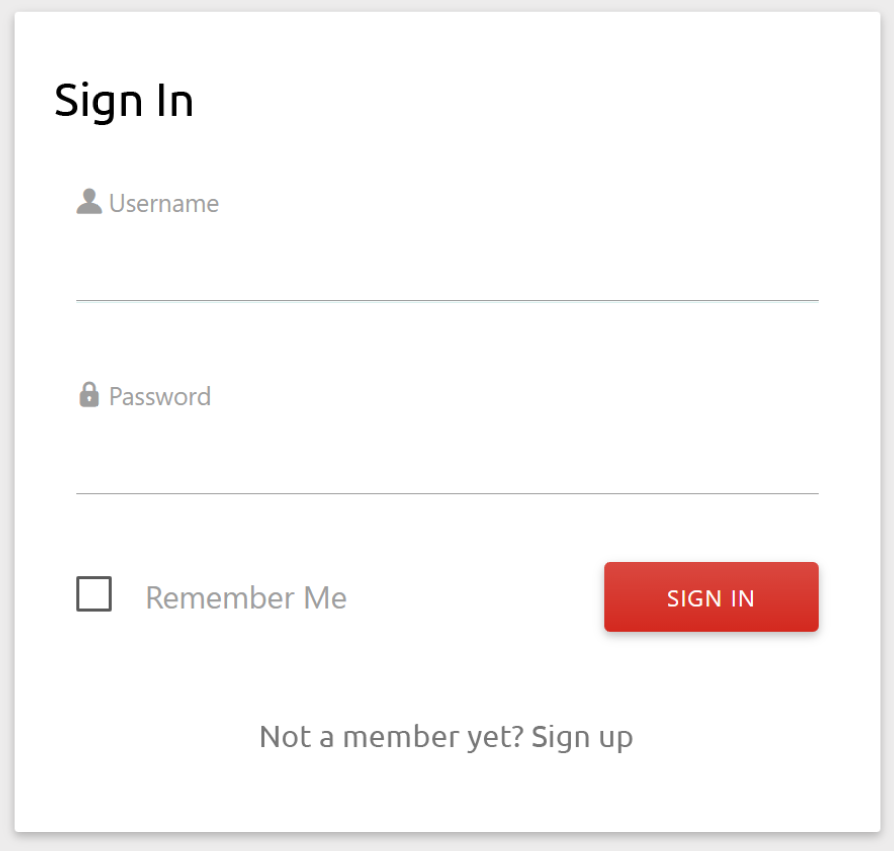
\includegraphics[width=0.75\textwidth]{signin}
\caption{Sign in page}
\end{figure}

\subsection{Registration}
All users must register in order to use ClinicFlow. Registration is simple, and requires only a username and password. \\
If you already have an account, please refer to Login (4.1) \\
To Sign Up:
\begin{enumerate}
\item Enter a desired username into the Username field (must be unique)
\item Enter a desired password into the Password field. It must meet the following requirements:
\begin{itemize}
	\item Between 8 and 20 characters
	\item Contain at least 1 number and 1 symbol
\end{itemize}
\item Click the "I am not a robot" checkbox.
\item Click "Sign up"
\end{enumerate}

\begin{figure}[H]
\centering
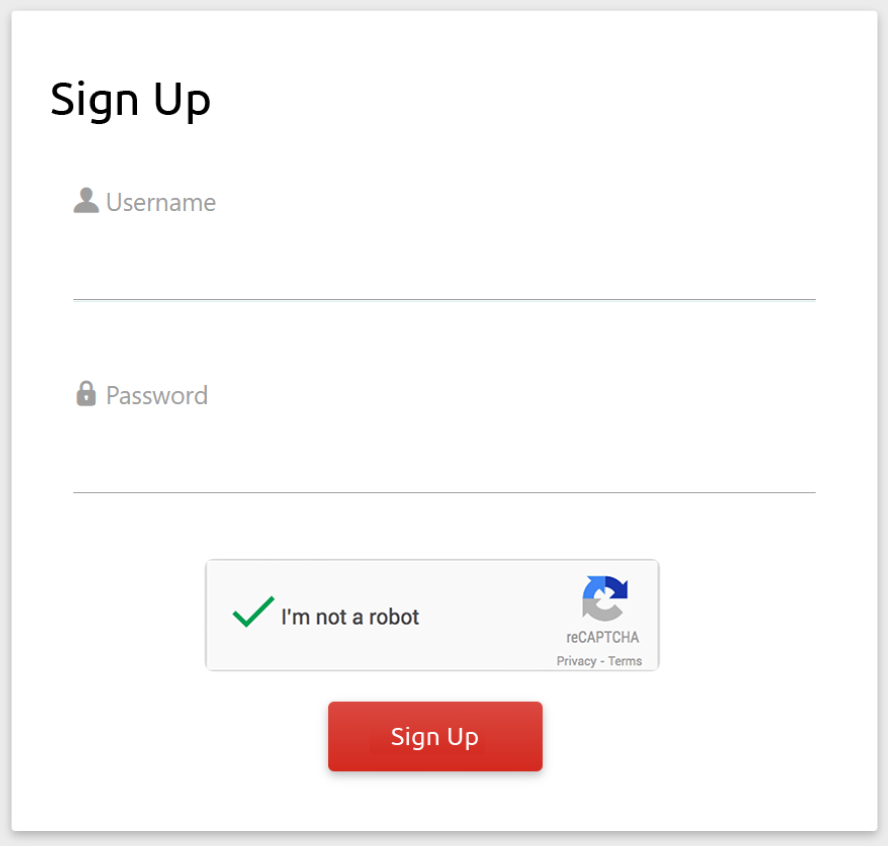
\includegraphics[width=0.8\textwidth]{signup}
\caption{Sign up page}
\end{figure}

\section{Dashboard}
\subsection{Clinic}
Upon logging in, the user will be presented the clinic selection screen. From here they can either select the clinic to use, or create a new clinic.\\

If no clinic is associated with this account, one must be created (See 5.1.1)\\

\subsubsection{Create Clinic}
To use this application, a clinic must be created it's constraints set up.\\
To create clinic, one must be on the "Choose Clinic screen" (See figure 4)\\

To create a clinic:
\begin{enumerate}
\item Click the "Create Clinic" button
\item Enter the clinic name (must be unique)
\item Enter clinic constraints
\begin{enumerate}
	\item Services: list the services available to the patients
	\item Providers: Set type and number of staff, including breaks and administered services
\end{enumerate}
\item Click "Create New Clinic"
\end{enumerate}
\begin{figure}[H]
\centering
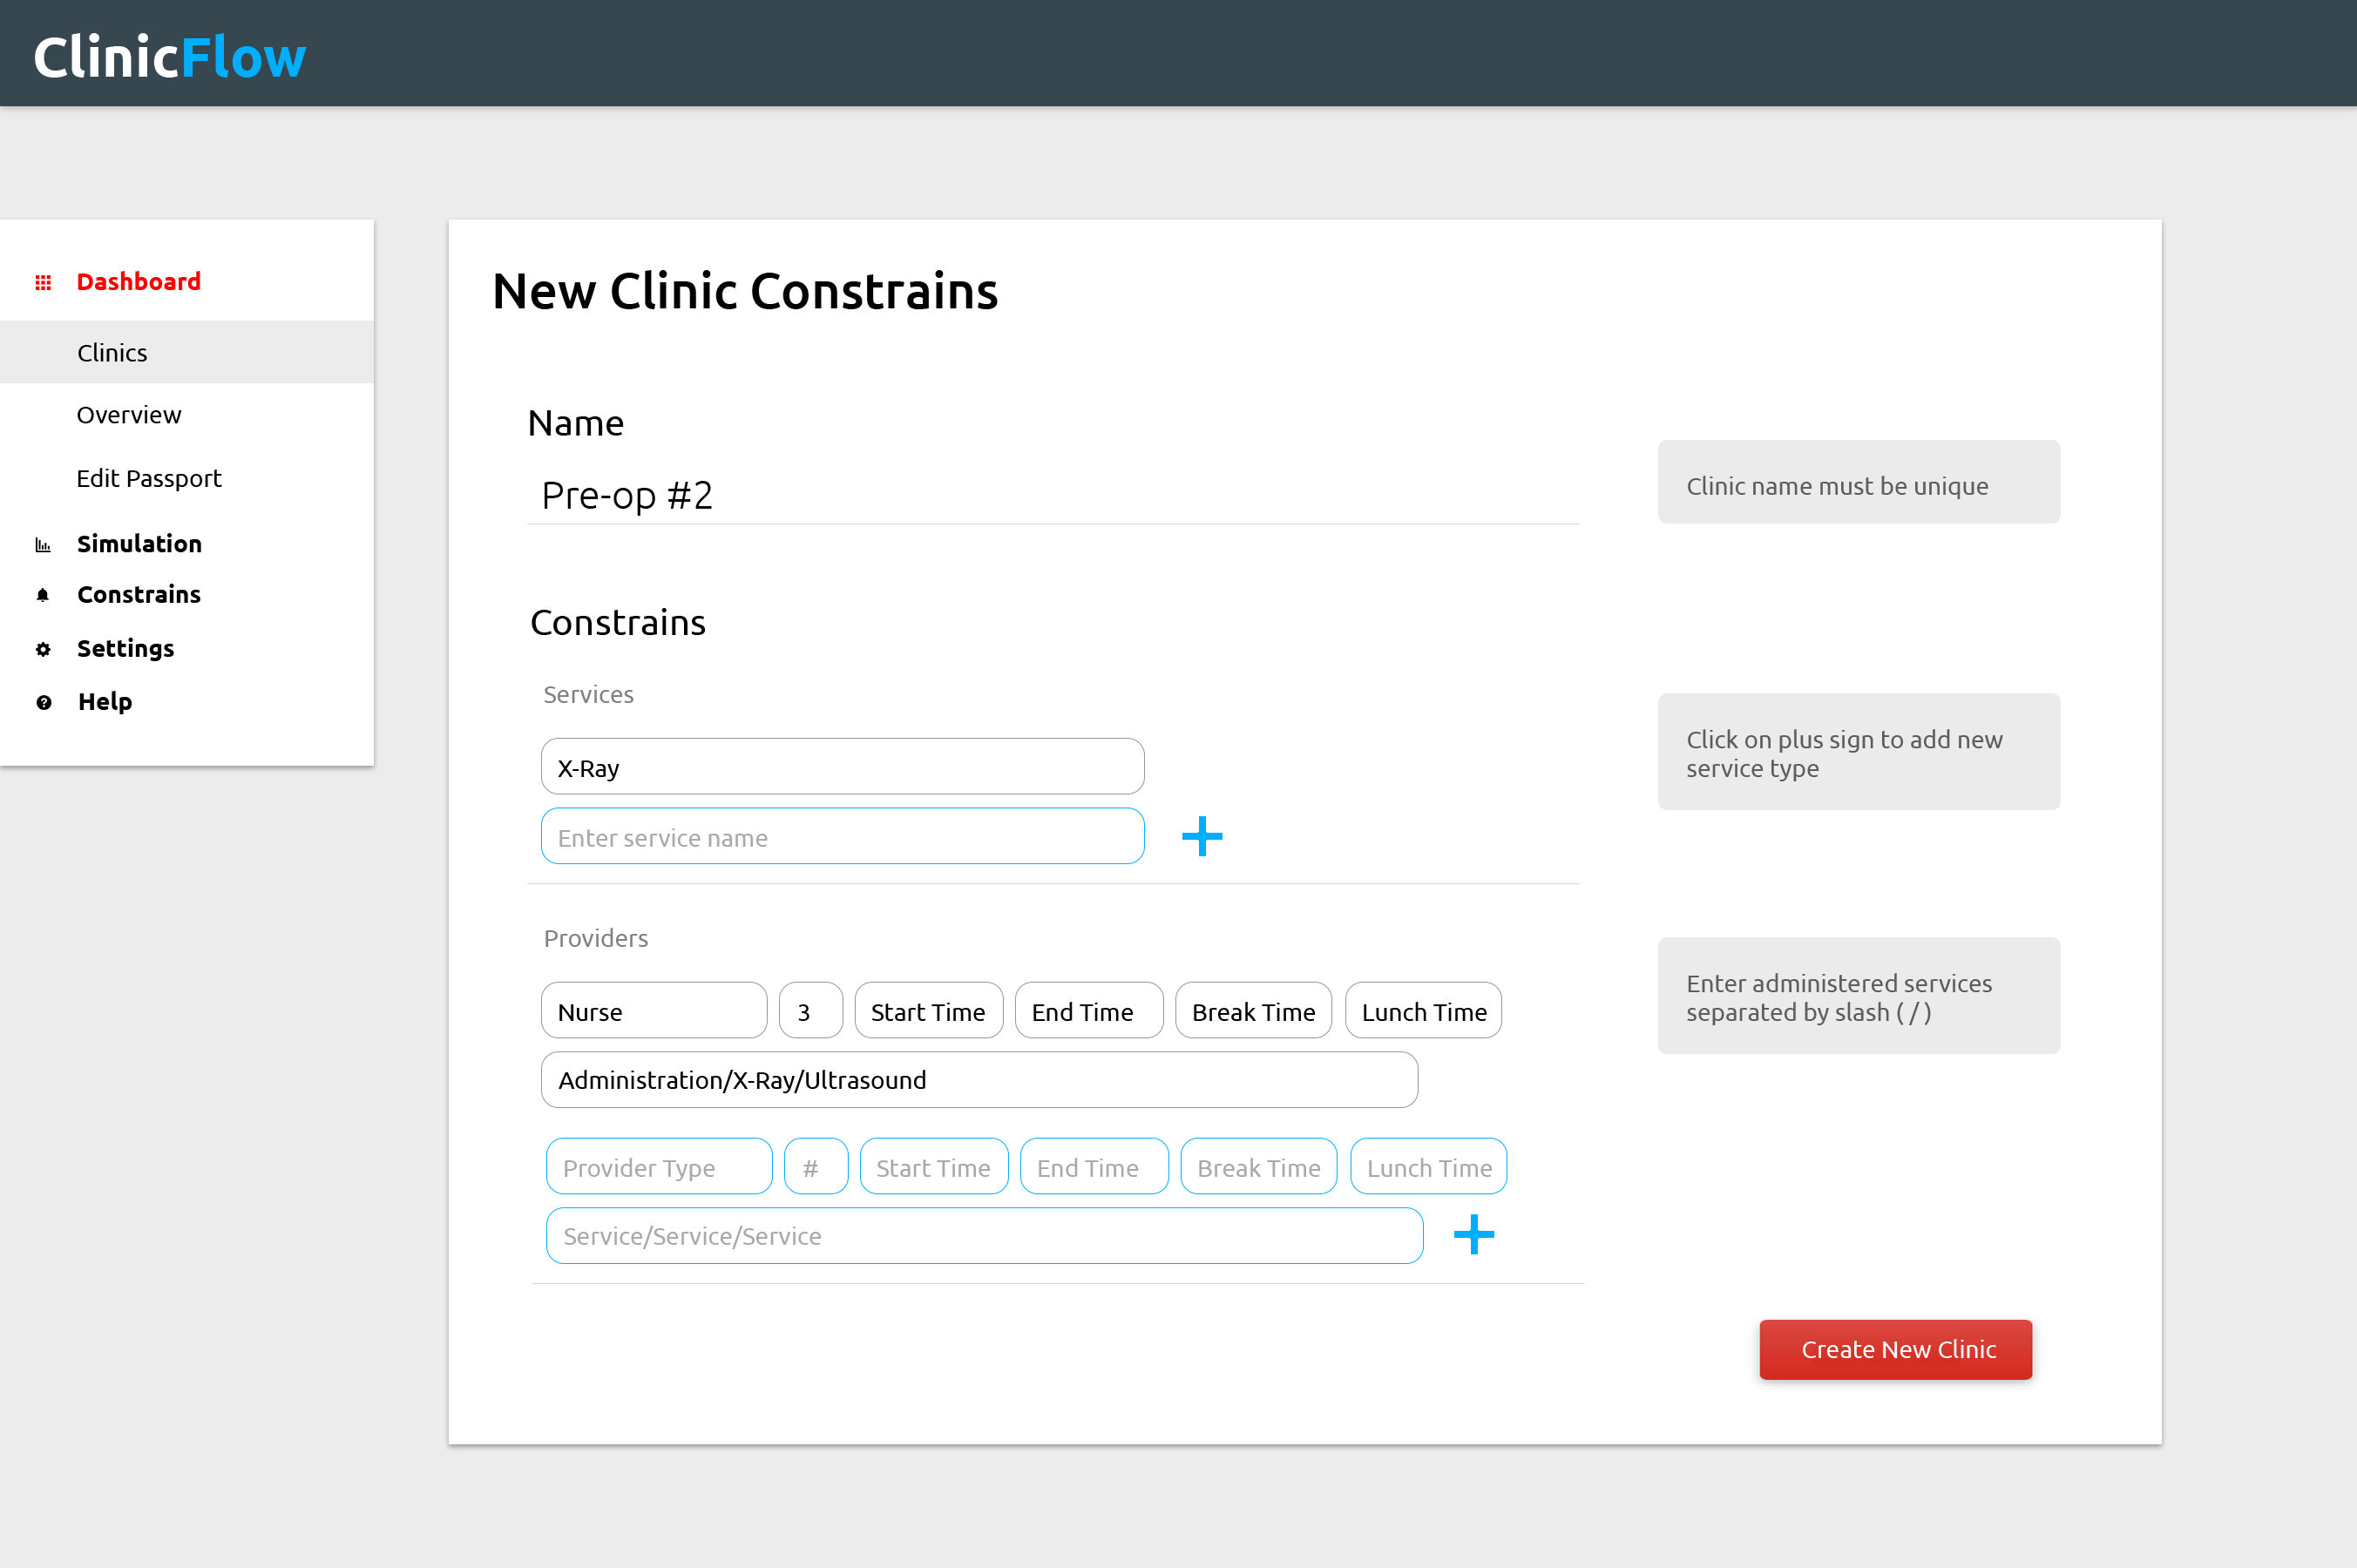
\includegraphics[width=\textwidth]{newclinic}
\caption{Creating a new clinics}
\end{figure}

\subsubsection{Select Clinic}
To select a clinic, click on one of the clinics in the list. (See figure X3)\\
Note: A clinic must be created in order to select a clinic (See 5.1.1)

\begin{figure}[H]
\centering
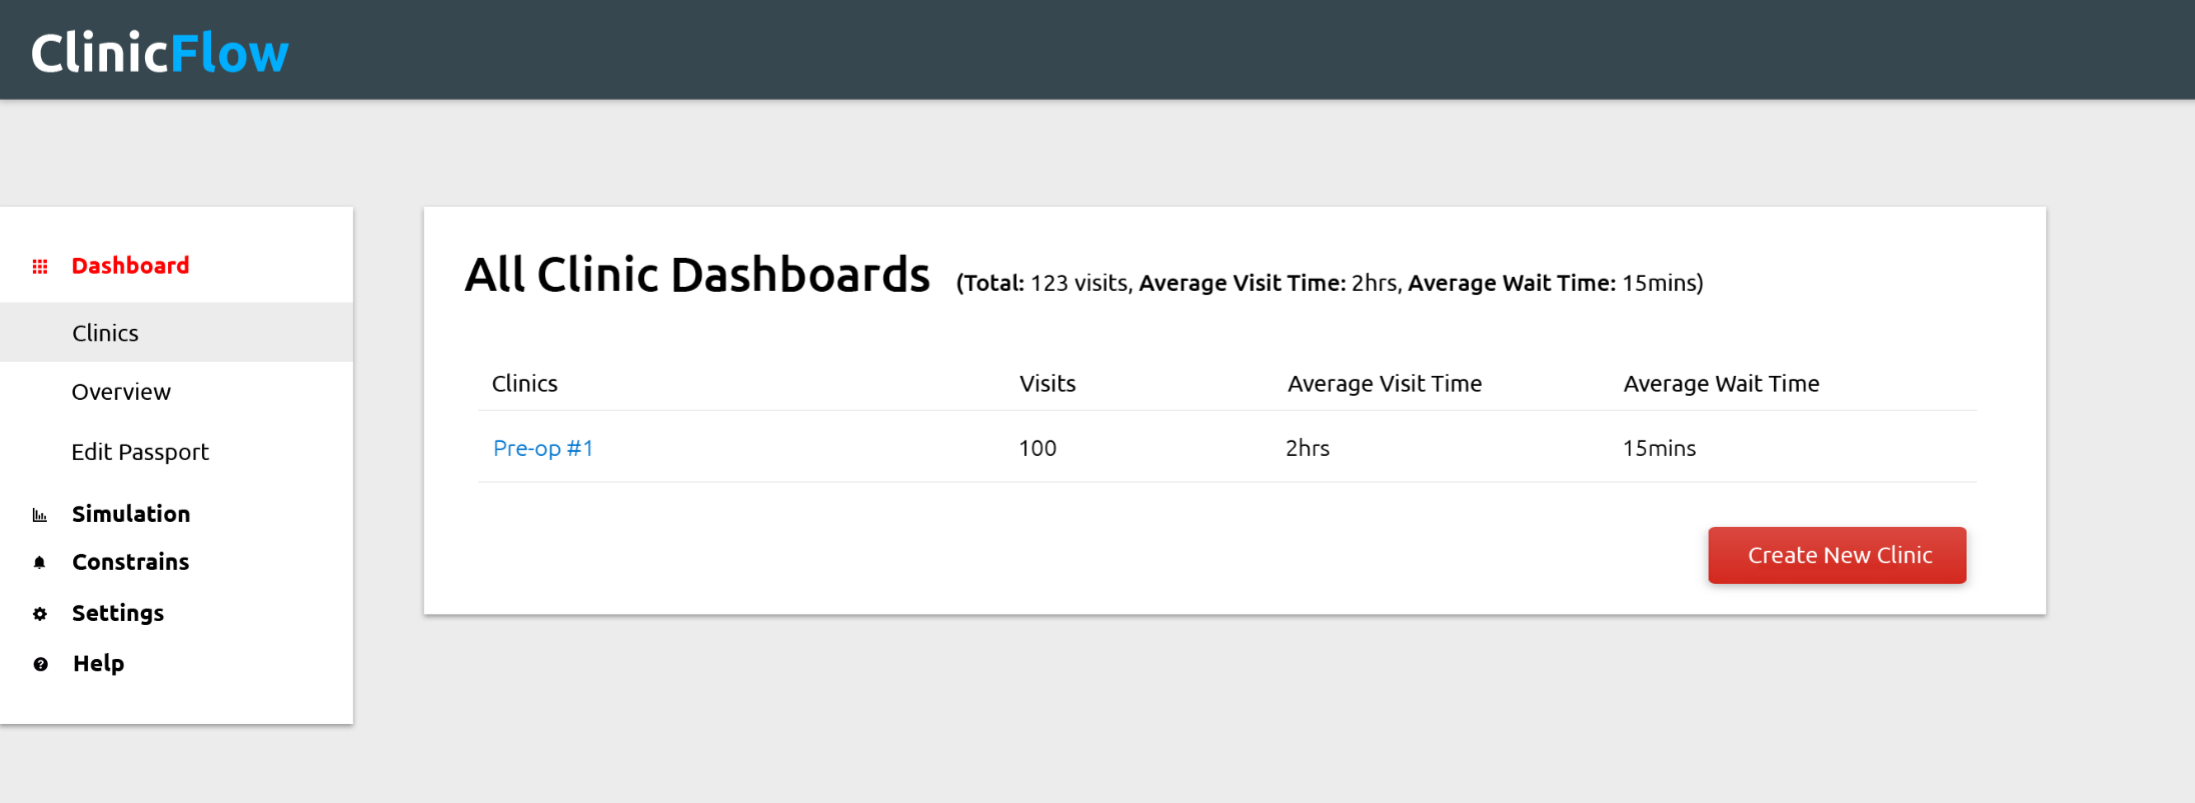
\includegraphics[width=\textwidth]{selectclinic}
\caption{Select from created clinics}
\end{figure}

\subsection{Overview}
This screen will show statistic about the current status of the clinic based on actual passport data.\\

Note: clinic passport data must be set up in order to use this screen (See 5.3)

\subsubsection{Select Date Range}
The selects the time range for which statistics will be calculated.\\
In order to change:
\begin{enumerate}
\item Click on the arrow beside the date at the top
\item Select the FROM date on the left
\item Select the TO date on the right
\item Click apply to filter the passport data to within that range
\pagebreak
\end{enumerate}

\begin{figure}[H]
\centering
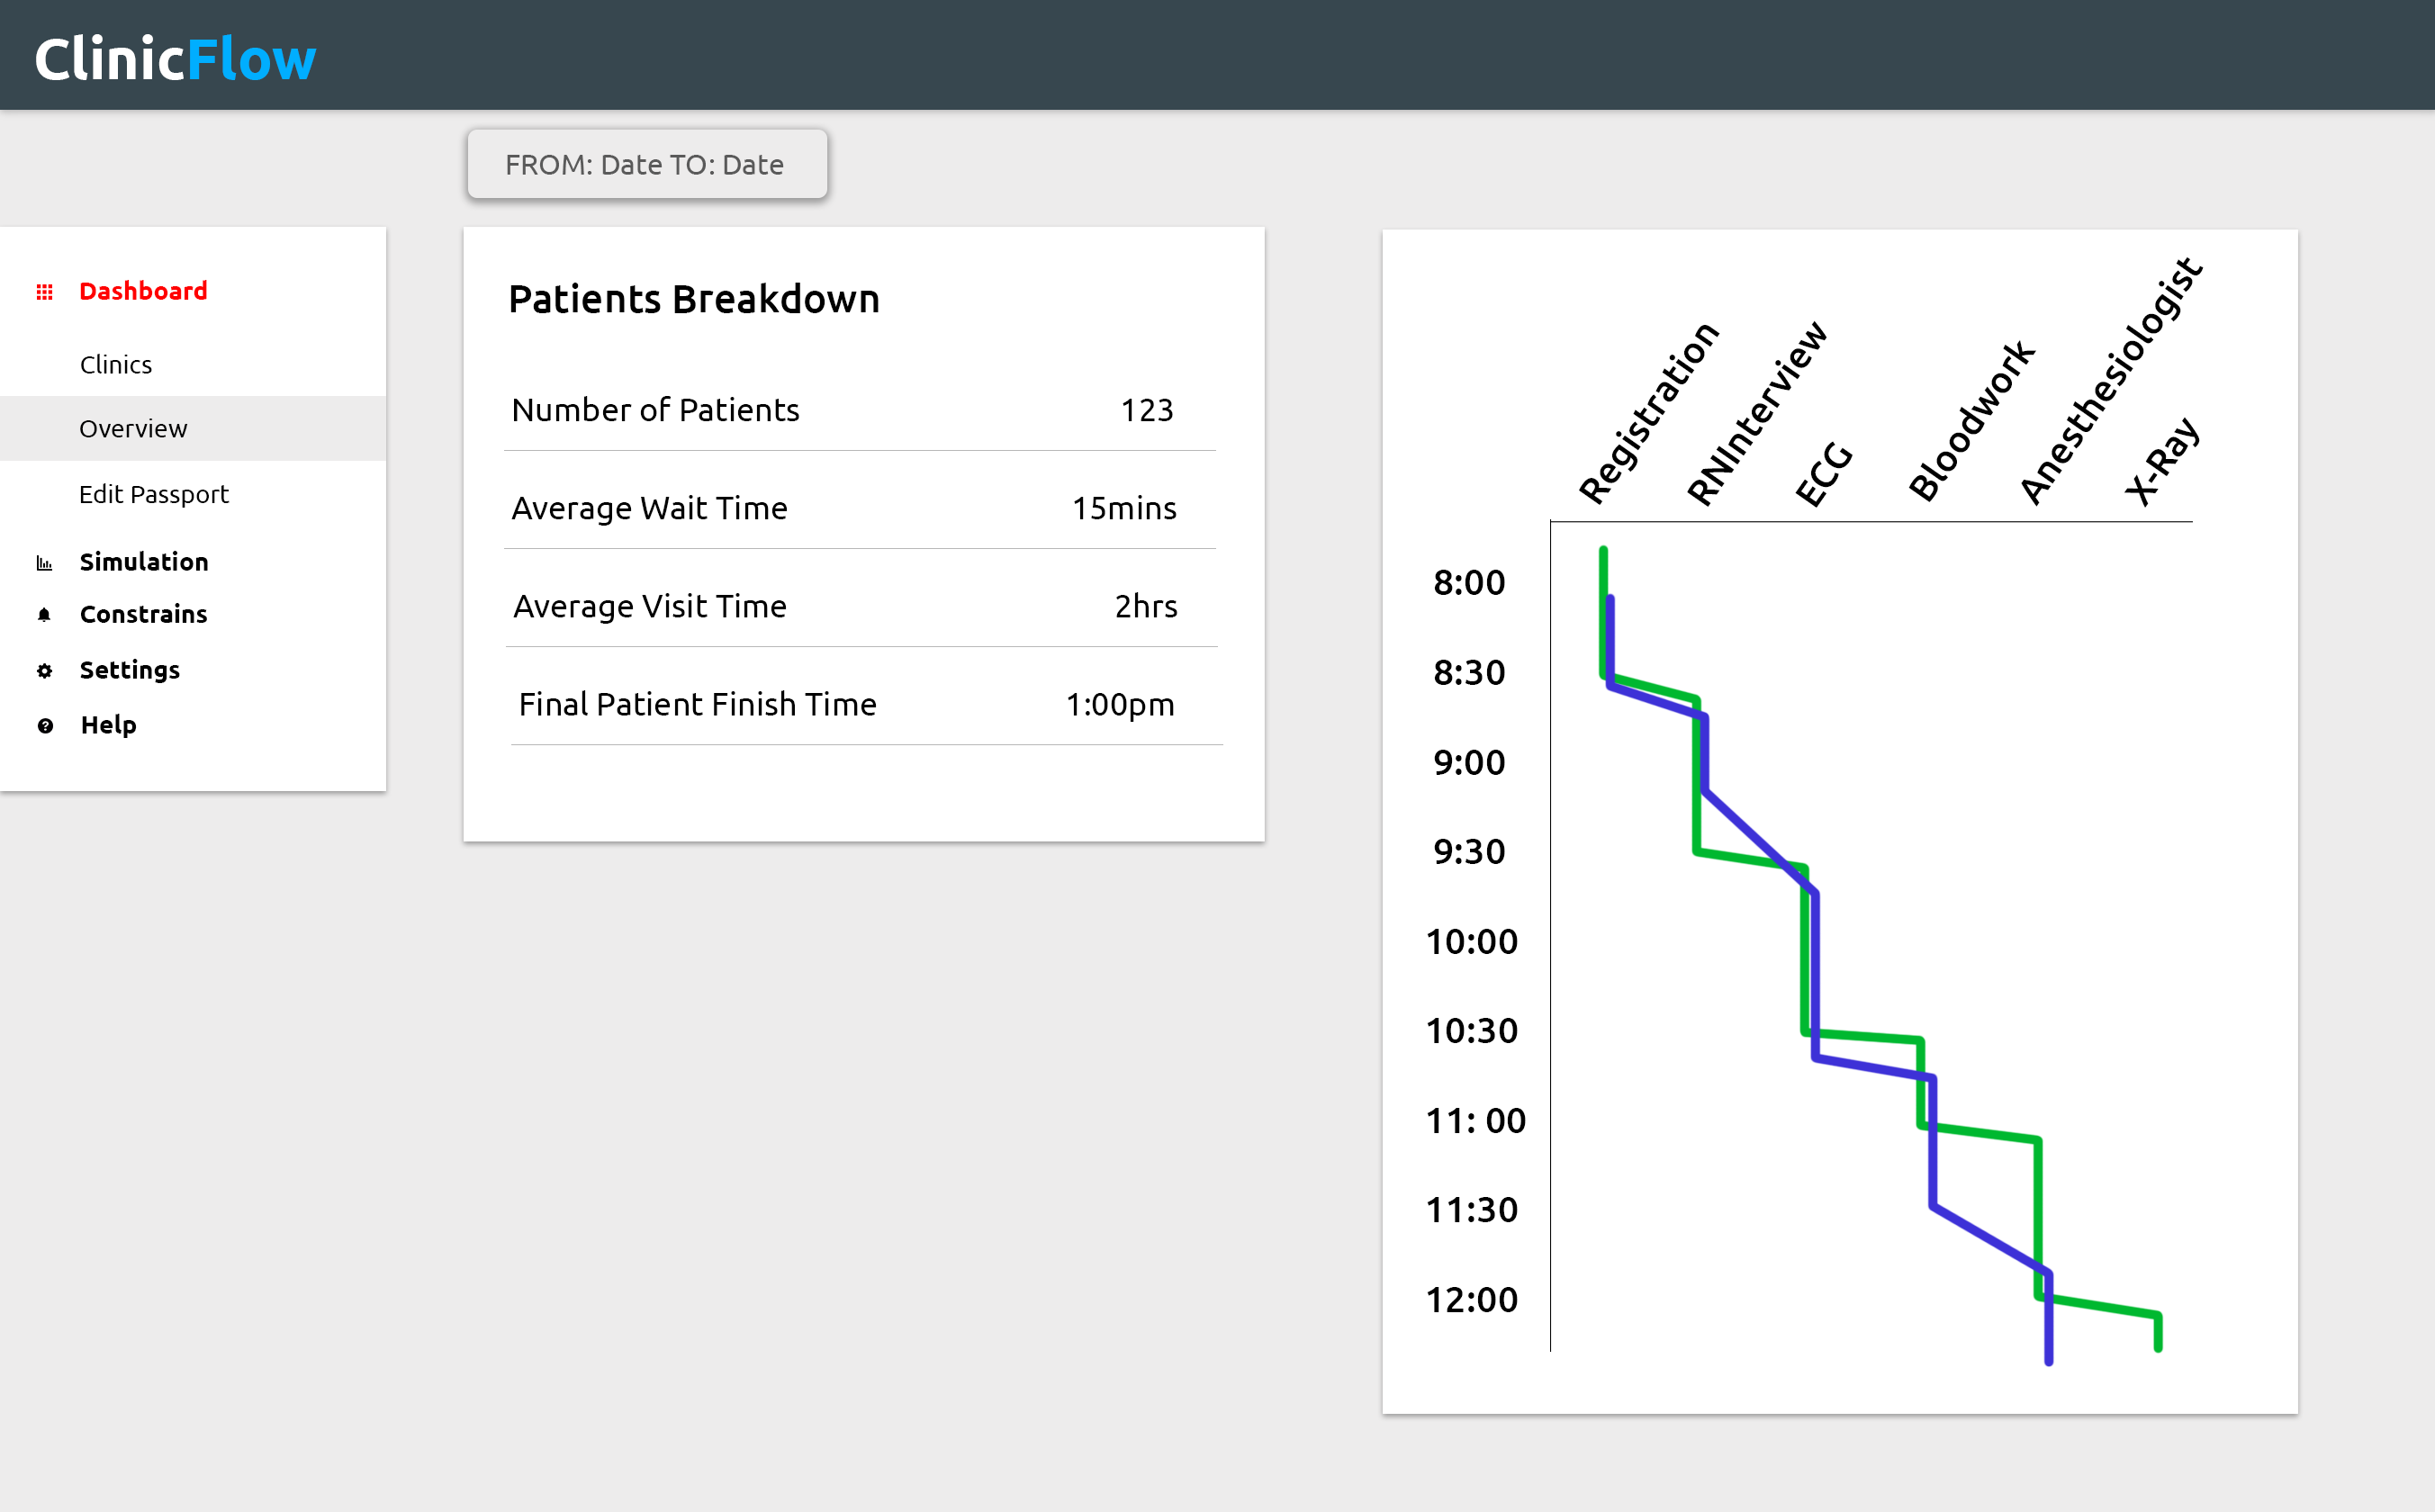
\includegraphics[width=\textwidth]{overview}
\caption{Overview of Clinic}
\end{figure}

\subsection{Edit Passport}
This section allow the user to edit past actual data. This data is used to provide summary statistics of the clinic environment, as well as help build a model of the clinic for simulation purposes. \\ \newline
Note: In order to edit passport, the clinic must have a set of constraints associated with it (See 5.5) \\
To add a patient:
\begin{enumerate}
\item Click the "Add patient" button
\item Enter the patient information, including name/id, scheduled arrival time, and required procedures
\item Click "Apply"
\end{enumerate}

To remove a patient:
\begin{enumerate}
\item Click the "X" button beside the patient name in the list
\item Click "Apply"
\end{enumerate}
\subsection{Simulate}
This section of the application allows the user to simulate a model clinic environment. \\
If no schedule/rule set has been created, the user must create one first (See 5.4.2) \\

\subsubsection{Simulation Selection}
This screen shows a list of stored simulation models. \\

To select a simulation, click on the name of simulation.

\subsubsection{Create Model}
This function allow the user to create a new simulation model. This is required in order to run simulations. \\

\begin{figure}[H]
\centering
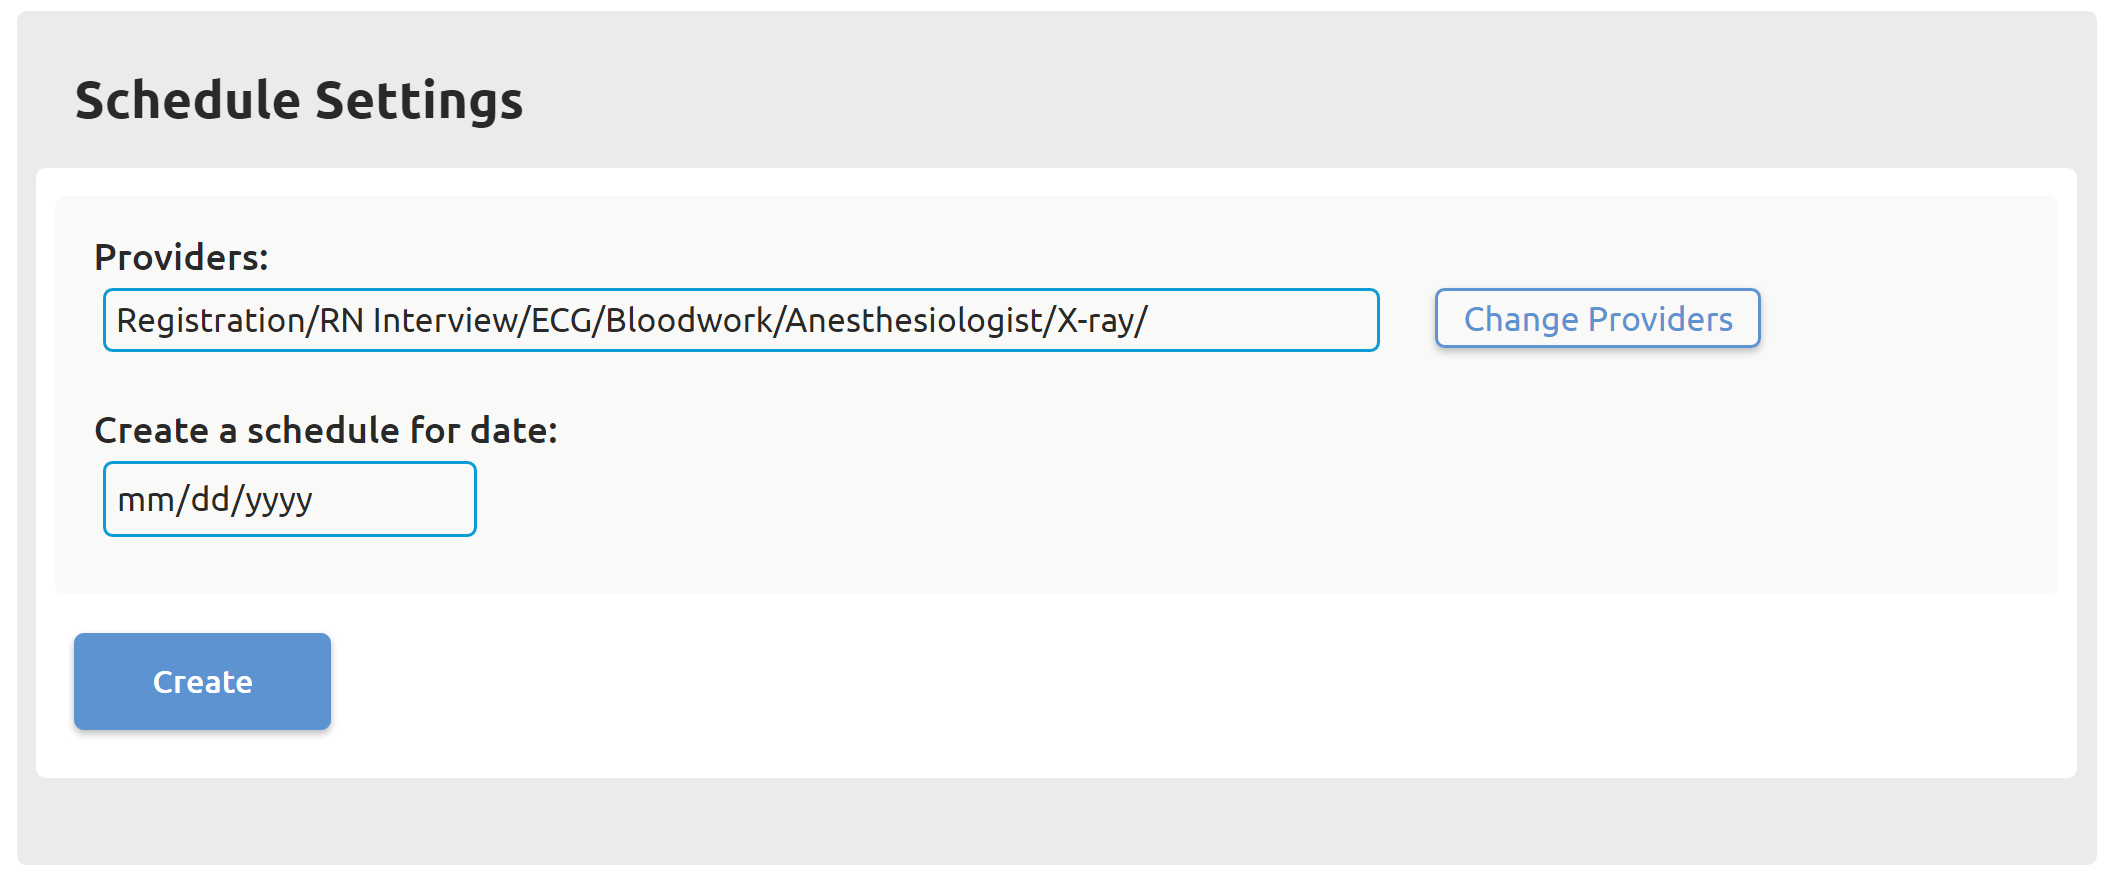
\includegraphics[width=\textwidth]{simsetting}
\caption{Creating simulation}
\end{figure}

To create a simulation model:
\begin{enumerate}
\item Click "Create Model"
\item Click "Use constraint info" (skip to 5) or Fill in details (steps 3-4)
\item Enter patients to simulate
\begin{enumerate}
\item Click "Add patient"
\item Enter name, arrival time, and required procedures
\end{enumerate}
\item Enter constraints to adhere to
\begin{enumerate}
\item Enter providers, staff, and prerequisites
\end{enumerate}
\item Click "Create"
\end{enumerate}

\begin{figure}[H]
\centering
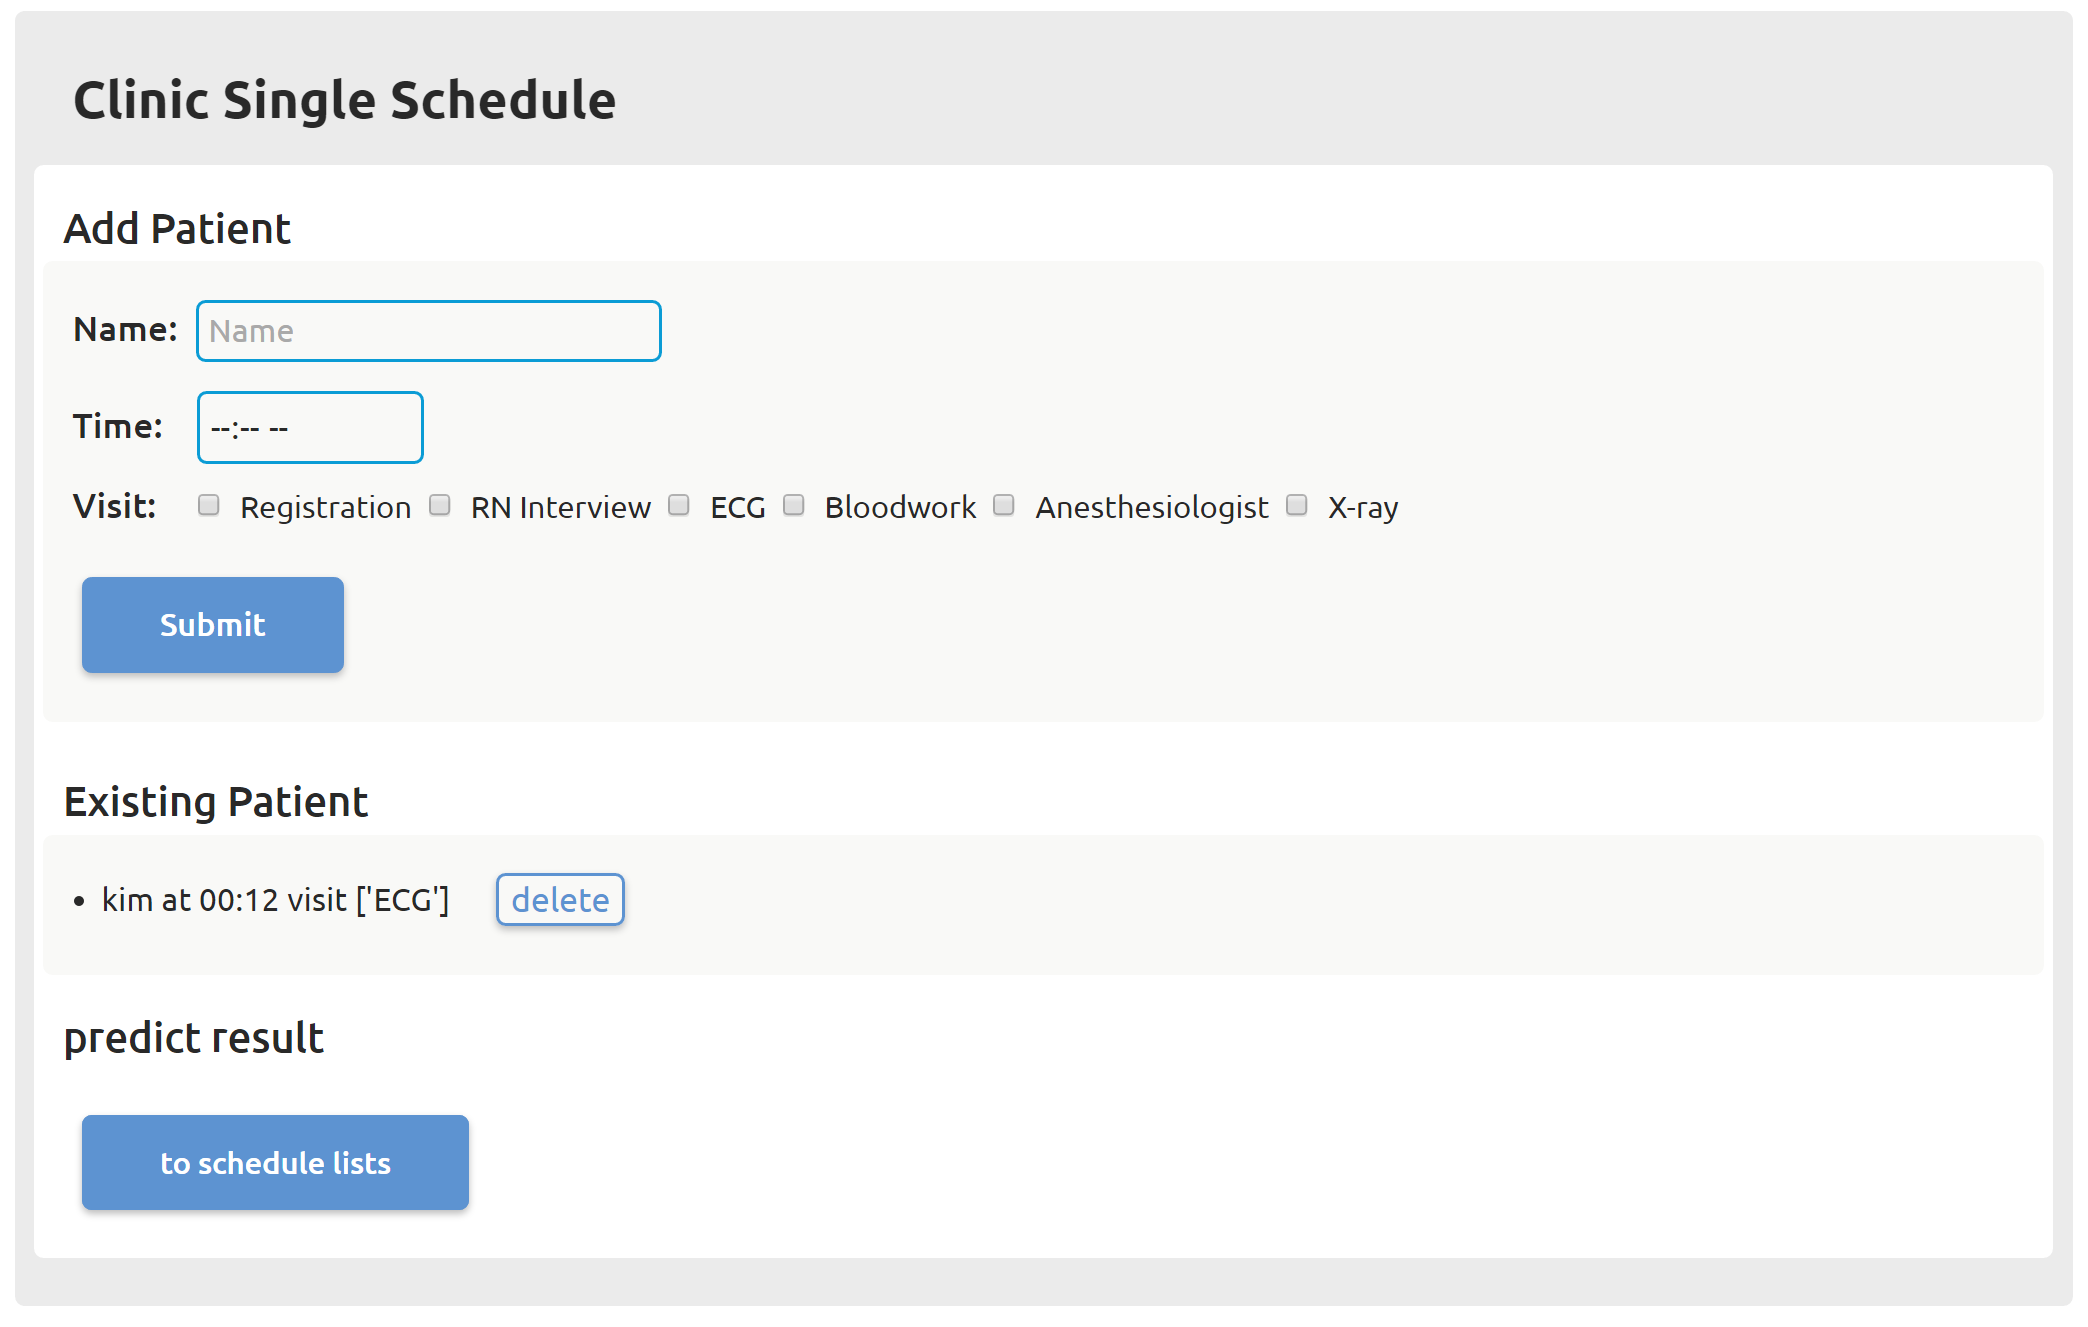
\includegraphics[width=\textwidth]{sim}
\caption{Add Patients to Simulation}
\end{figure}

\subsubsection{Results}
This screen shows statistics from the last simulation. If no simulation has been performed, only the simulation selection screen will be visible.\\

In order to simulate a model, click on the "Simulate" button beside the model in the list.\\

The results screen shows statistics such as mean procedure time, waiting time, total clinic operation time. \\

\subsection{Constraints}
This section allows the user to change the constraints for the current clinic.\\

All 3 sections must have their properties set in order to use the passport feature, as well as to use constraint info in a simulation model.\\

\subsubsection{Change Providers / prerequisites / staff}
This section allow the user to set the list of providers available in the clinic.\\

In order to add a provider:
\begin{enumerate}
\item Click the "+" button under "Providers" to add an additional provider.
\item  Enter the name of the provider in the new text box
\item Click Apply to save the list of providers
\end{enumerate}

In order to set the prerequisites:\\
\begin{enumerate}
\item Click the "+" button under "Prerequisites" to add a prerequisite
\item Enter the before procedure
\item Enter the after procedure
\item Click "Apply' to save the list of prerequisites
\end{enumerate}

In order to set the staff:
\begin{enumerate}
\item Click the "+" button under "Staff" to add a staff member
\item Enter their name
\item Enter the procedures they can provide
\item Enter their start, end, and break times.
\item Click "Apply" to save the list of staff
\end{enumerate}

\subsection{Settings}
This section allows the user to change setting related to their account

\subsubsection{Change Password}
The user can change the password for their account: \\
\begin{enumerate}
\item Click on "Change Password"
\item  Enter current password
\item Enter current password again
\item  Enter new password
\item  Click "Apply"
\end{enumerate}
\subsubsection{Change Clinic Name}
The user can change the name of any clinic associated with their account
To do this: \\
\begin{enumerate}
\item Click "Change clinic name"
\item  Select clinic whose name to change
\item Enter new name for clinic
\item Click "Apply"
\end{enumerate}

\section{Troubleshooting}
\subsection{FAQ}
This section provides information on commonly asked questions regarding the operation of product. \\
\begin{enumerate}
\item  Why do I not see a list of clinics?
\begin{itemize}
\item You must be signed in, and have at least 1 clinic create in order to see the list of clinics. See 4.1, 5.1.1.
\end{itemize}

\item  Why do I not see a passport?
\begin{itemize}
\item You must enter the clinic constraints and patient data in order to see the passport and statistics. See 5.5, 5.3
\end{itemize}
\end{enumerate}
\subsection{Contact Us}
If you have any further questions contact us at:
\begin{itemize}
\item huw7@mcmaster.ca
\item vasiliem@mcmcaster.ca
\item knopfk@mcmaster.ca
\item yum27@mcmaster.ca
\item li544@mcmaster.ca
\end{itemize}

\section{Definitions}
\begin{itemize}
\item Account:  An entity identified by username and password credentials. Contains clinics. 
\item Clinic: An entity consisting of a passport and constraints.
\item Passport: A spreadsheet of past clinic data, including patient arrival time, procedure duration, and departure time.
\item Constraints: Rules regarding clinic behavior, used in simulation
\end{itemize}
\end{document}
